\section{Das Environment}

Als Environment für diese Experimentreihe wollen wir eine Gebirgslandschaft erzeugen, über der ein Raster liegt, worauf sich der Agent bewegen kann. Hierbei soll jeder Punkt auf dem Raster eine Höhe besitzen. Außerdem soll die Landschaft zufällig generiert werden können.

Die simpelste Lösung hierfür wäre wohl, ein zweidimensionales Array mit zufälligen Zahlen zu füllen. Auf diese Weise erhält man ein für jede Koordinate eine zufällige Höhe. Wir wollen allerdings für die intuitive Auswertung der Experimente (zum Beispiel \glqq Hat der Agent einen Berg gefunden?\grqq) eine Landschaft erstellen, die organisch und natürlich aussieht.

% \subsection{Perlin Noise}
\paragraph{Perlin Noise}
Um dieses Ziel zu erreichen verwenden wir \textit{Perlin Noise} (\cite{parberry2015modeling}). Hierbei handelt es sich um eine Rauschfunktion, mit der sich sehr natürlich wirkende Texturen zufällig generieren lassen. Abbildung \ref{img:perlinNoise} zeigt eine simple Darstellung von zweidimensionalem Perlin Noise, bei der die generierten Werte über Farbwerten von Schwarz bis Weiß abgebildet werden.

\begin{figure}[H]
    \centering
    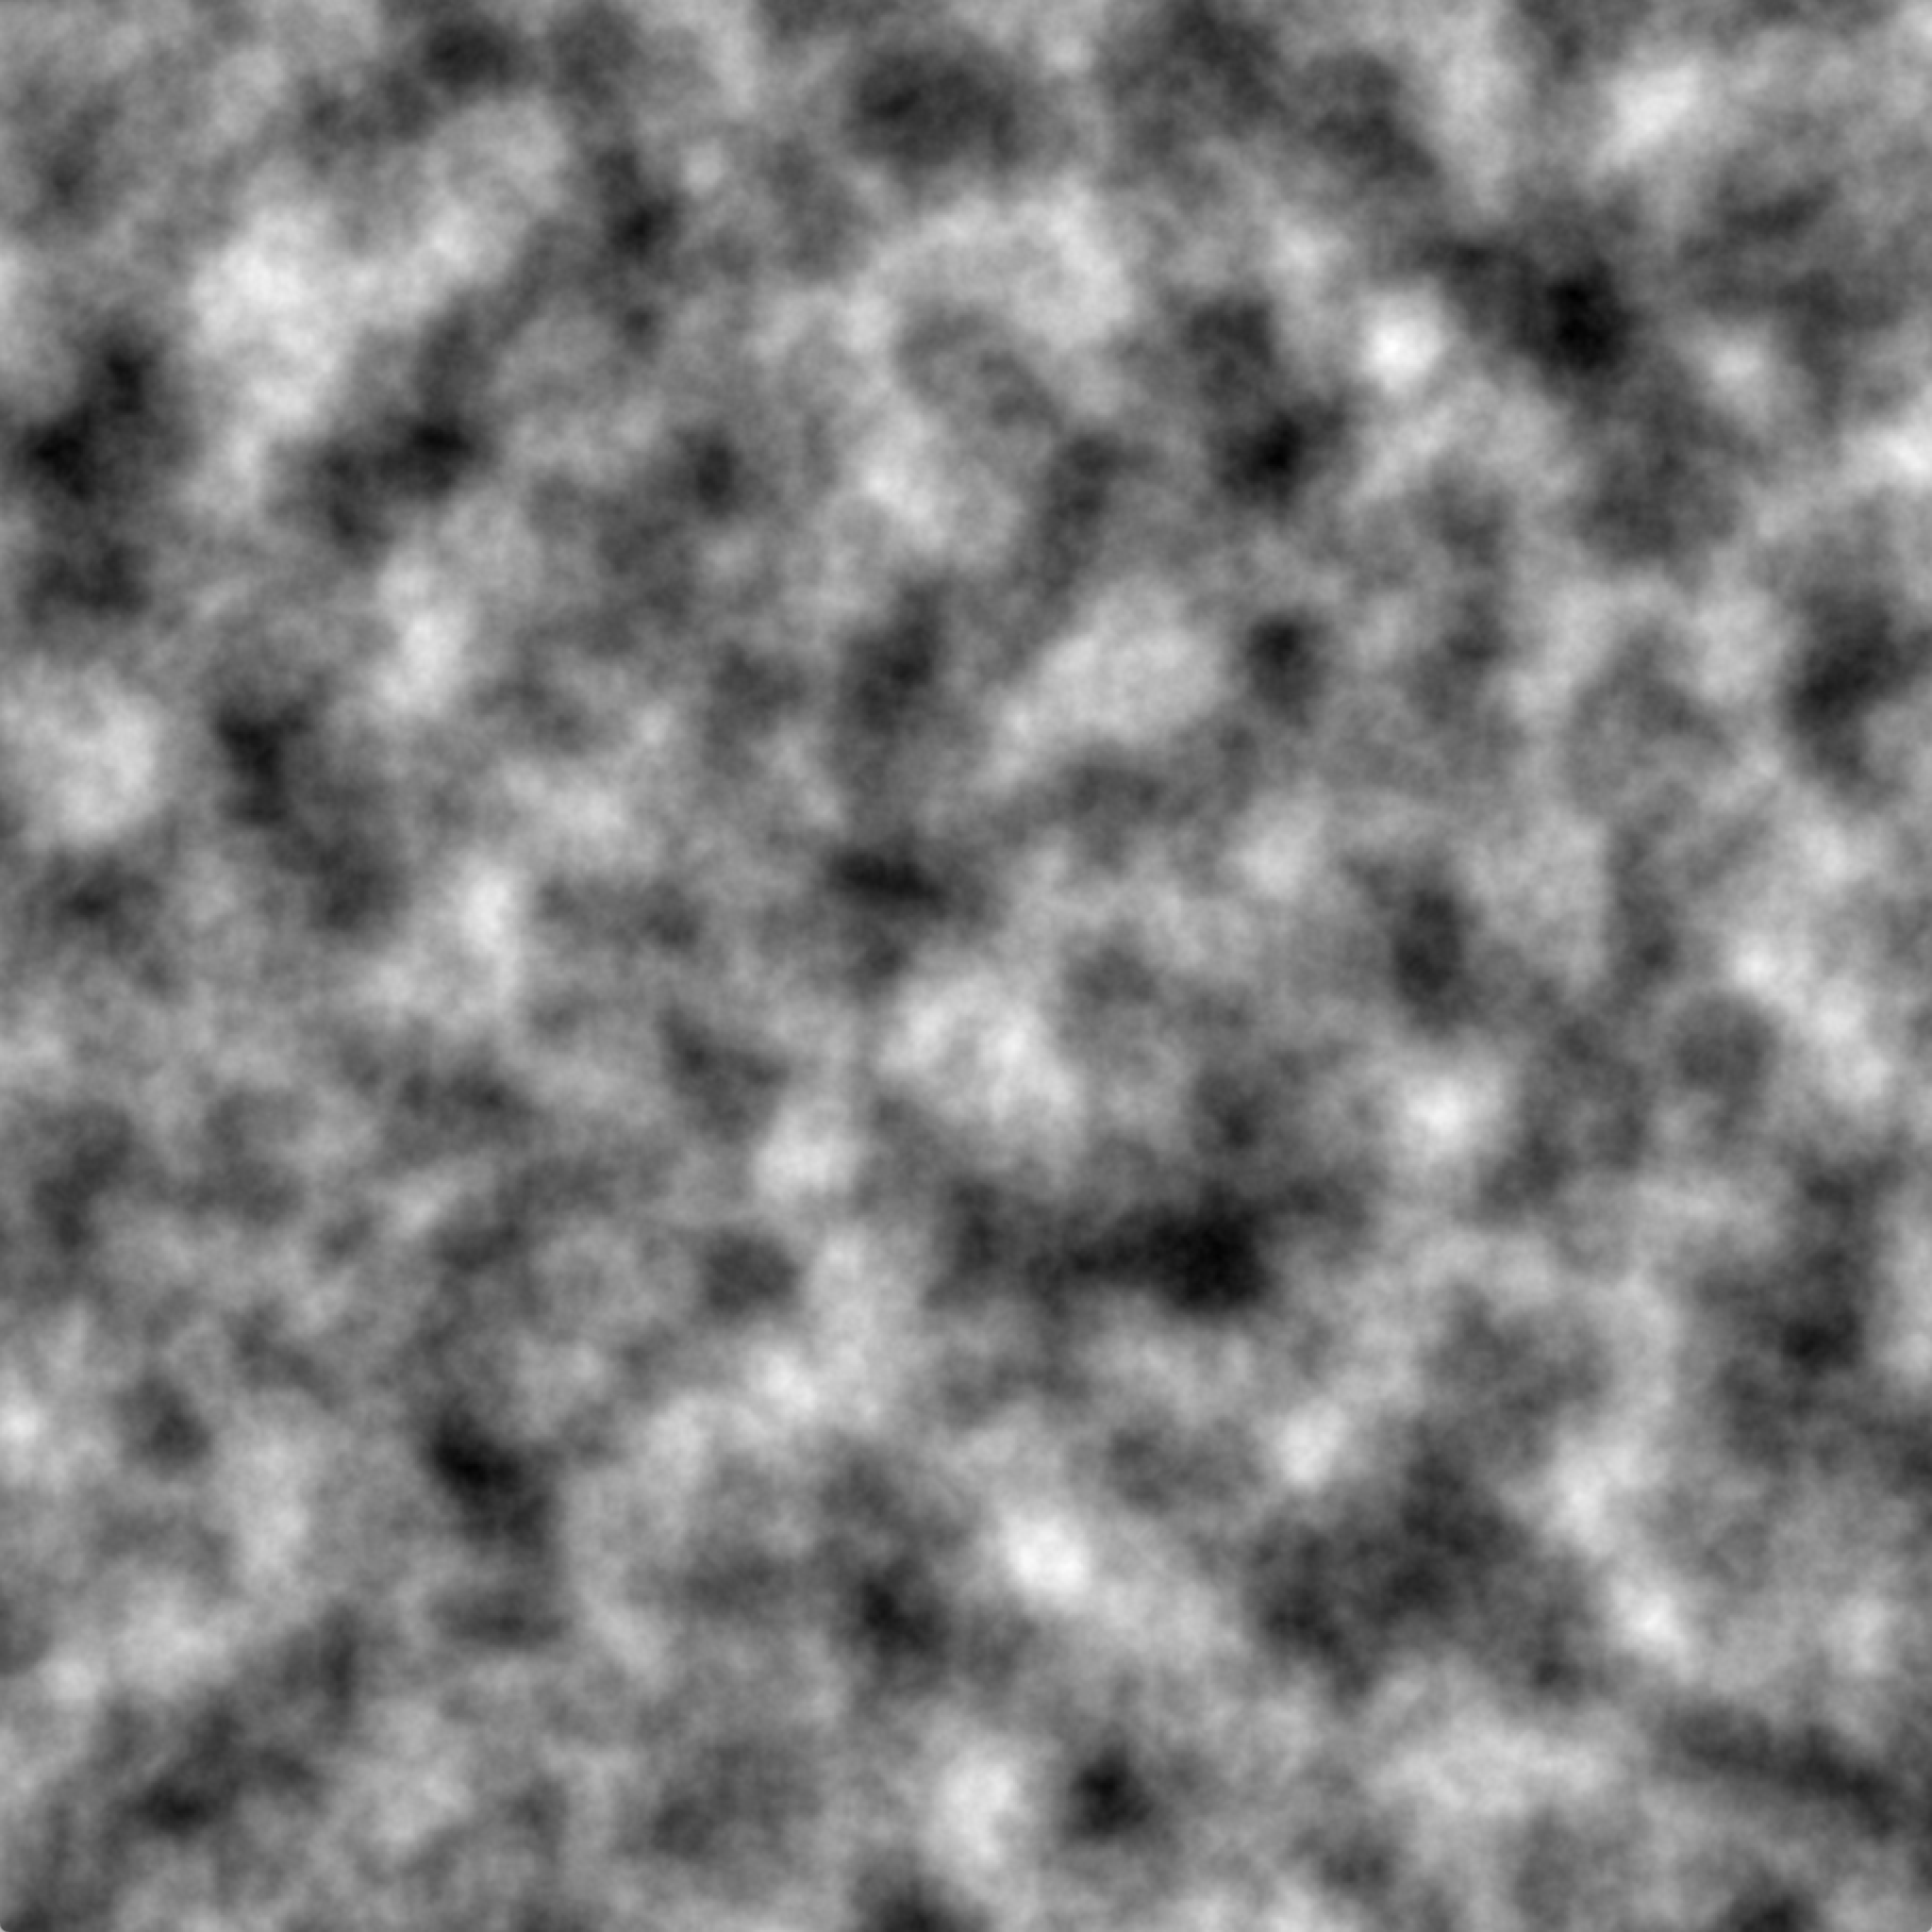
\includegraphics[width=0.5\textwidth, keepaspectratio=true]{perlin_noise.png}
    \caption{Visualisierung von zweidimensionaler Perlin Noise} \label{img:perlinNoise}
    \source{\url{https://miro.medium.com/max/2400/1*vs239SecVBaB4HvLsZ8O5Q.png}}
\end{figure}

% TODO evtl weiter ausführen
% Bei Initialisierung der Klasse werden zunächst $ x \cdot y $ Gradienten erstellt, wobei $ x $ und $ y $ entweder der Länge und der Breite des Rasters entsprechen, oder einem Bruchteil dessen, um gewissermaßen in das Rauschen \glqq hereinzuzoomen \grqq{}.

% \begin{minted}{python}
% class PerlinNoise:

%     def __init__(self, x, y):
%         x, y = math.ceil(x) + 1, math.ceil(y) + 1
%         self.gradients = []
%         for j in range(y):
%             self.gradients.append([])
%             for i in range(x):
%                 a = random.uniform(0, 1)
%                 b = math.sqrt(1 - a ** 2)
%                 c = [-1, 1][random.randint(0, 1)]
%                 d = [-1, 1][random.randint(0, 1)]
%                 self.gradients[j].append([a * c, b * d])
% \end{minted}

Perlin Noise ist nach \cite{parberry2015modeling} ein fundamentaler Algorithmus in der prozeduralen Generierung von Terrain und somit optimal geeignet, um unsere Umgebung zu erstellen. Wir verwenden eine modifizierte Implementierung von TODO, um ein zweidimensionales Array mit zufälligen Werten zwischen -1 und 1 zu erhalten, welche wir mit einer beliebigen Höhe multiplizieren können. Je nachdem, wie stark man in die Rauschfunktion \glqq hereinzoomt\grqq{} erhält man unterschiedliche Verteilungen der Landschaft, wie man in Abbildung \ref{img:randomTerrain} erkennen kann.

\begin{figure}[H]
    \centering
    \begin{subfigure}[b]{0.49\textwidth}
        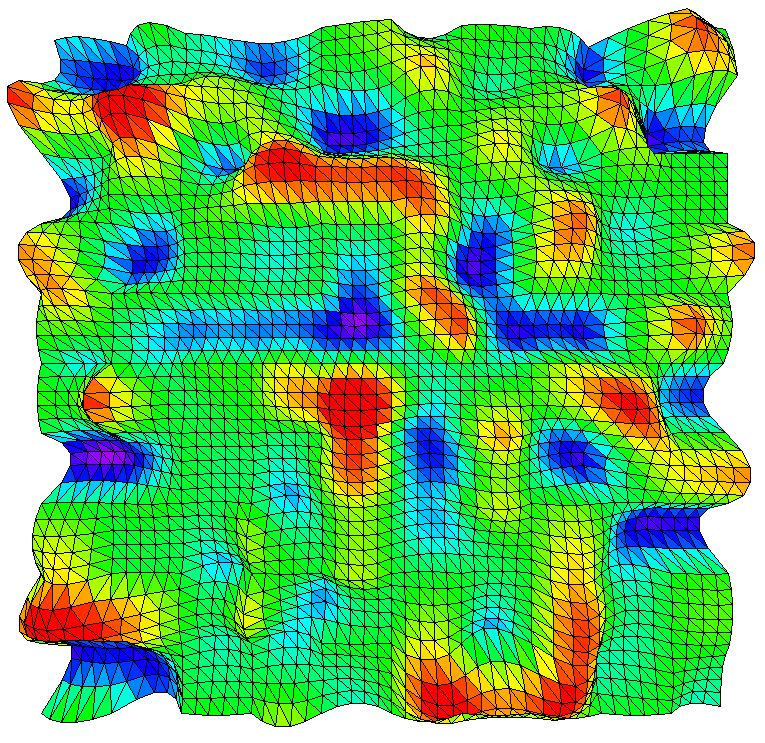
\includegraphics[width=\textwidth]{terrain_01.JPG}
        \caption{Landschaft mit niedriger Verteilung}
        \label{img:randomTerrainA}
    \end{subfigure}
    \begin{subfigure}[b]{0.49\textwidth}
        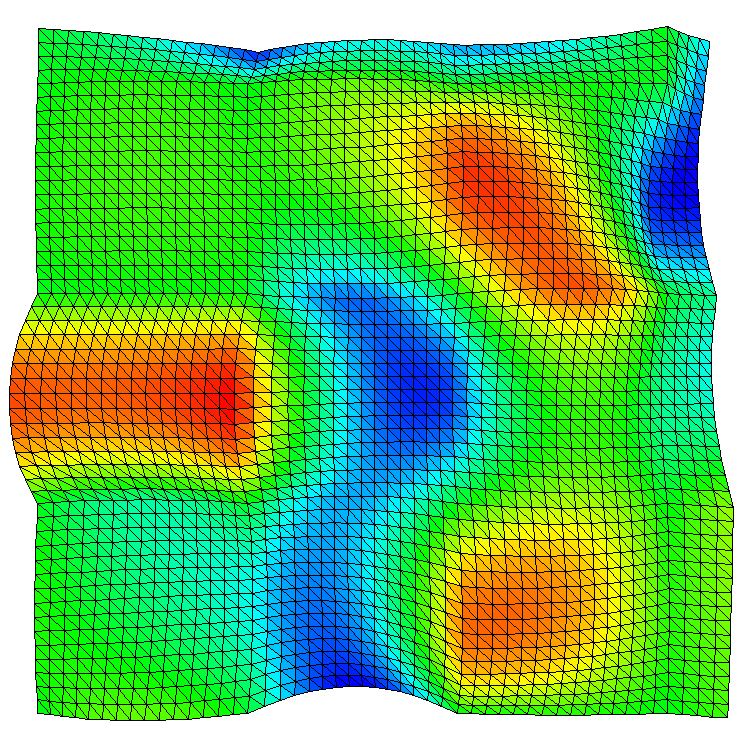
\includegraphics[width=\textwidth]{terrain_02.JPG}
        \caption{Landschaft mit hoher Verteilung}
        \label{img:randomTerrainB}
    \end{subfigure}
    \caption{Mittels Perlin Noise zufällig generierte Landschaften}
    \label{img:randomTerrain}
    % \subfigure[Figur A]{terrain_01.JPG}
    % \subfig[Figur A]{ \label{img:randomTerrainA}
    %     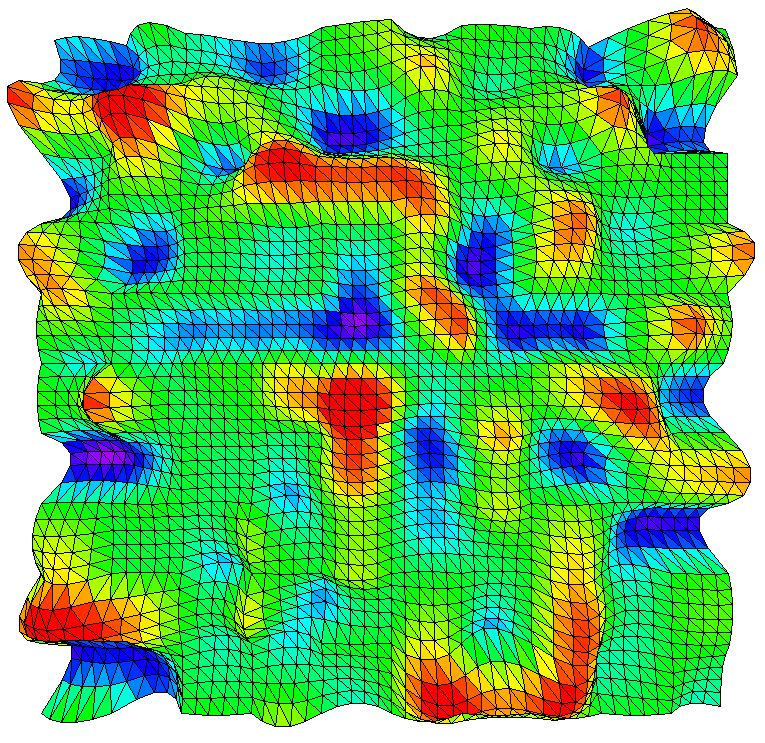
\includegraphics[width=0.95\textwidth]{terrain_01.JPG}
    % }
    % \captionabove{Test}
        % \begin{subfigure}{0.5\textwidth}
        % 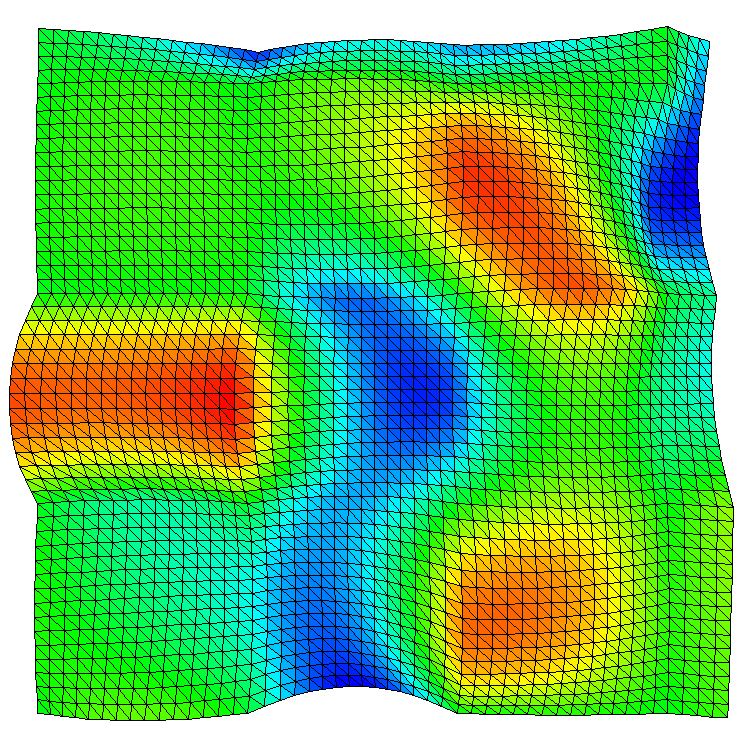
\includegraphics[width=0.95\textwidth, right]{terrain_02.JPG}
        % \caption{Zeitweilig überlagernde Fähigkeiten} \label{img:diayn_ex2}
        % \end{subfigure}
\end{figure}

Wir werden nicht näher auf die Details der Funktion eingehen, da dies nicht Kern dieser Arbeit ist. Für weitere Ausführungen diesbezüglich verweisen wir auf \cite{archer2011procedurally}.

Für die Visualisierung der Landschaft benutzen wir eine abgewandelte Form des Codes von TODO. Zur besseren Differenzierung werden Berge und Täler zusätzlich zur perspektivischen Unterscheidung rot bzw. blau dargestellt.

\smallspace

Wir besitzen nun die Möglichkeit, eine zufällige Landschaft zu generieren und diese visuell darzustellen. Um bei allen Experimenten die gleichen Vorraussetzungen zu gewährleisten, werden wir im Folgenden das mittels der eben beschriebenen Methode zufällig generierten Terrain benutzen, der in Abbildung \ref{img:terrainMain} zu sehen ist. Der höchste Punk befindet sich bei dieser Landschaft auf dem Berg ganz oben in der Mitte.

\begin{figure}[H]
    \centering
    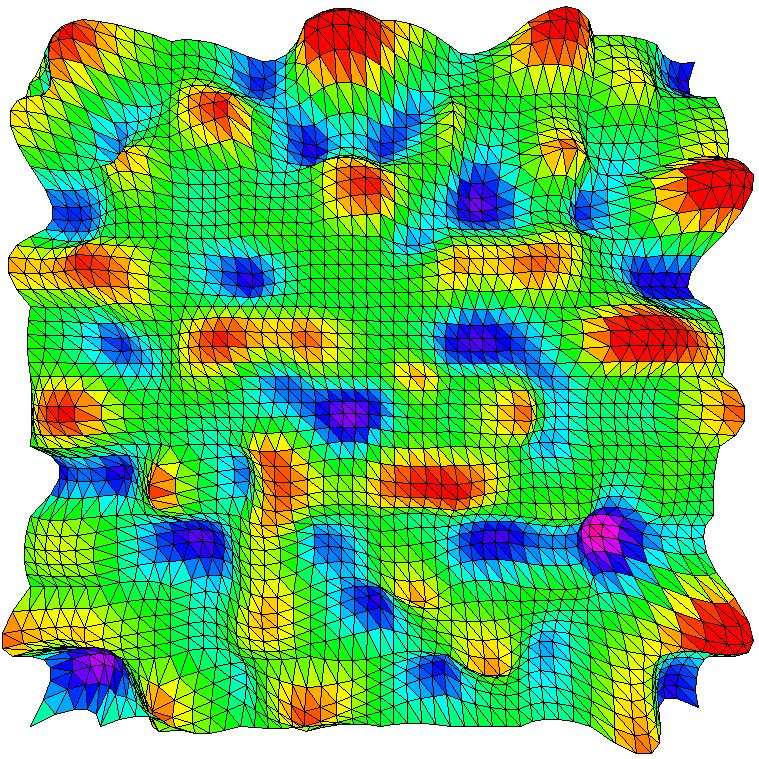
\includegraphics[width=0.5\textwidth, keepaspectratio=true]{terrain_main.JPG}
    \caption{TODO Main Terrain} \label{img:terrainMain}
\end{figure}